%%%%%%%%%%%%%%%%%%%%%%%%%%%%%%%%%%%%%%%%%%%%%%%%
% chapter1.tex                                 %
% Contains formatting and content of chapter 1 %
%%%%%%%%%%%%%%%%%%%%%%%%%%%%%%%%%%%%%%%%%%%%%%%%
\chapter{Name of Chapter}
\newpage

\section{Section Name 1}
Blah blah blah. Here is an example of how to include and cite a figure: see Figure~\ref{fig:example_figure}
\begin{figure}[H]
\center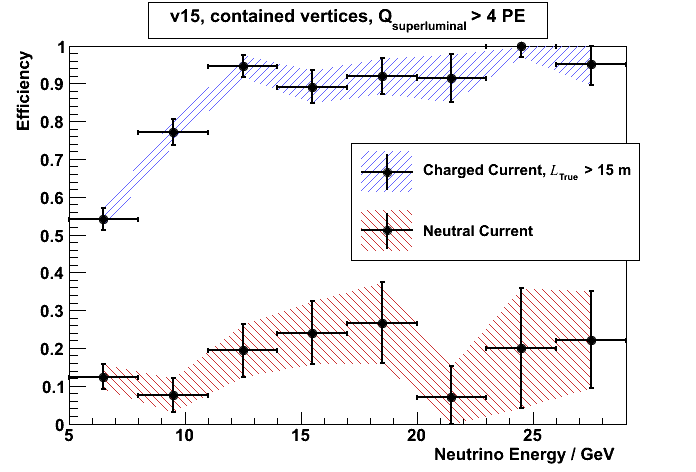
\includegraphics[width=0.4\textwidth]{figures/ExampleFigure.png}
\caption[Caption to go in list of figures]{Caption to go underneath figure}
\label{fig:example_figure}
\end{figure}

\section{Section Name 2}
Blah blah blah Here's an example of a table: see Table~\ref{tab:best_values}.

\begin{table}[H]
\centering\onehalfspacing
\vline
\begin{tabular}{c c c}
\hline
\textbf{Parameter} & \vline & \textbf{Current Best Value}\\
\hline
$\Delta m^2_{21}$ & \vline & $7.50^{+0.19}_{-0.20} \times 10^{-3}\;\mathrm{eV}^2$\\
$|\Delta m^2_{32}|$ & \vline & $2.32^{+0.12}_{-0.08} \times 10^{-5}\;\mathrm{eV}^2$\\
$\sin^2{(\theta_{12})}$ & \vline & $0.857^{+0.023}_{-0.025}$\\
$\sin^2{(2\theta_{23})}$ & \vline & $>0.95$\\
$\sin^2{(\theta_{13})}$ & \vline &  $0.098\pm 0.013$\\
\hline\end{tabular}\vline
\captionsetup{width=0.86\textwidth}
\caption[Name of table for list of tables]{Name of table for caption above table}
\label{tab:best_values}
\end{table}

Here's an example of an equation and some math:
\begin{equation}
  U = \begin{pmatrix} c_{12}c_{13} & s_{12}c_{13} & s_{13}e^{i\delta}\\
    -s_{12}c_{23} - c_{12}s_{23}s_{13}e^{i\delta} & c_{12}c_{23} - s_{12}s_{23}s_{13}e^{i\delta} & s_{23}c_{13}\\
    s_{12}s_{23} - c_{12}c_{23}s_{13}e^{i\delta} & -c_{12}s_{12} - s_{12}c_{23}s_{13}e^{i\delta} & c_{23}c_{13}
  \end{pmatrix},
\end{equation}
with $c_{ij} = \cos{\theta_{ij}}$ and $s_{ij} = \sin{\theta_{ij}}$.

Here's an example citation: \citep{PDG}.